\section{Goales}


\textbf{Emotional Goal} Make the inner-workings of a deep learning system accessible for organisation. And play with one!\\


\textbf{Destiney} Finally build one Deep Learning Network!

Technical goal (1): Be able to "data science it". Using cloud application (via) iPad\\

Technical goal (2): Build a deep learning image recognition or something cooler or more applicable to the first emotional goal, but don't jump back and forth. 


\section{Setting Up Jupyter Notebook instance on AWS Stage Maker}

\paragraph{Goal: Running it on iPad}

A specialltiy will be, that this will be done on an iPad with \textit{Juno Connect}. Also this section follows the guide from  \url{https://youtu.be/pqs5u2FKtu8?si=Som8aY_IrXLLNI_m}

\begin{figure}[H]
	\centering
	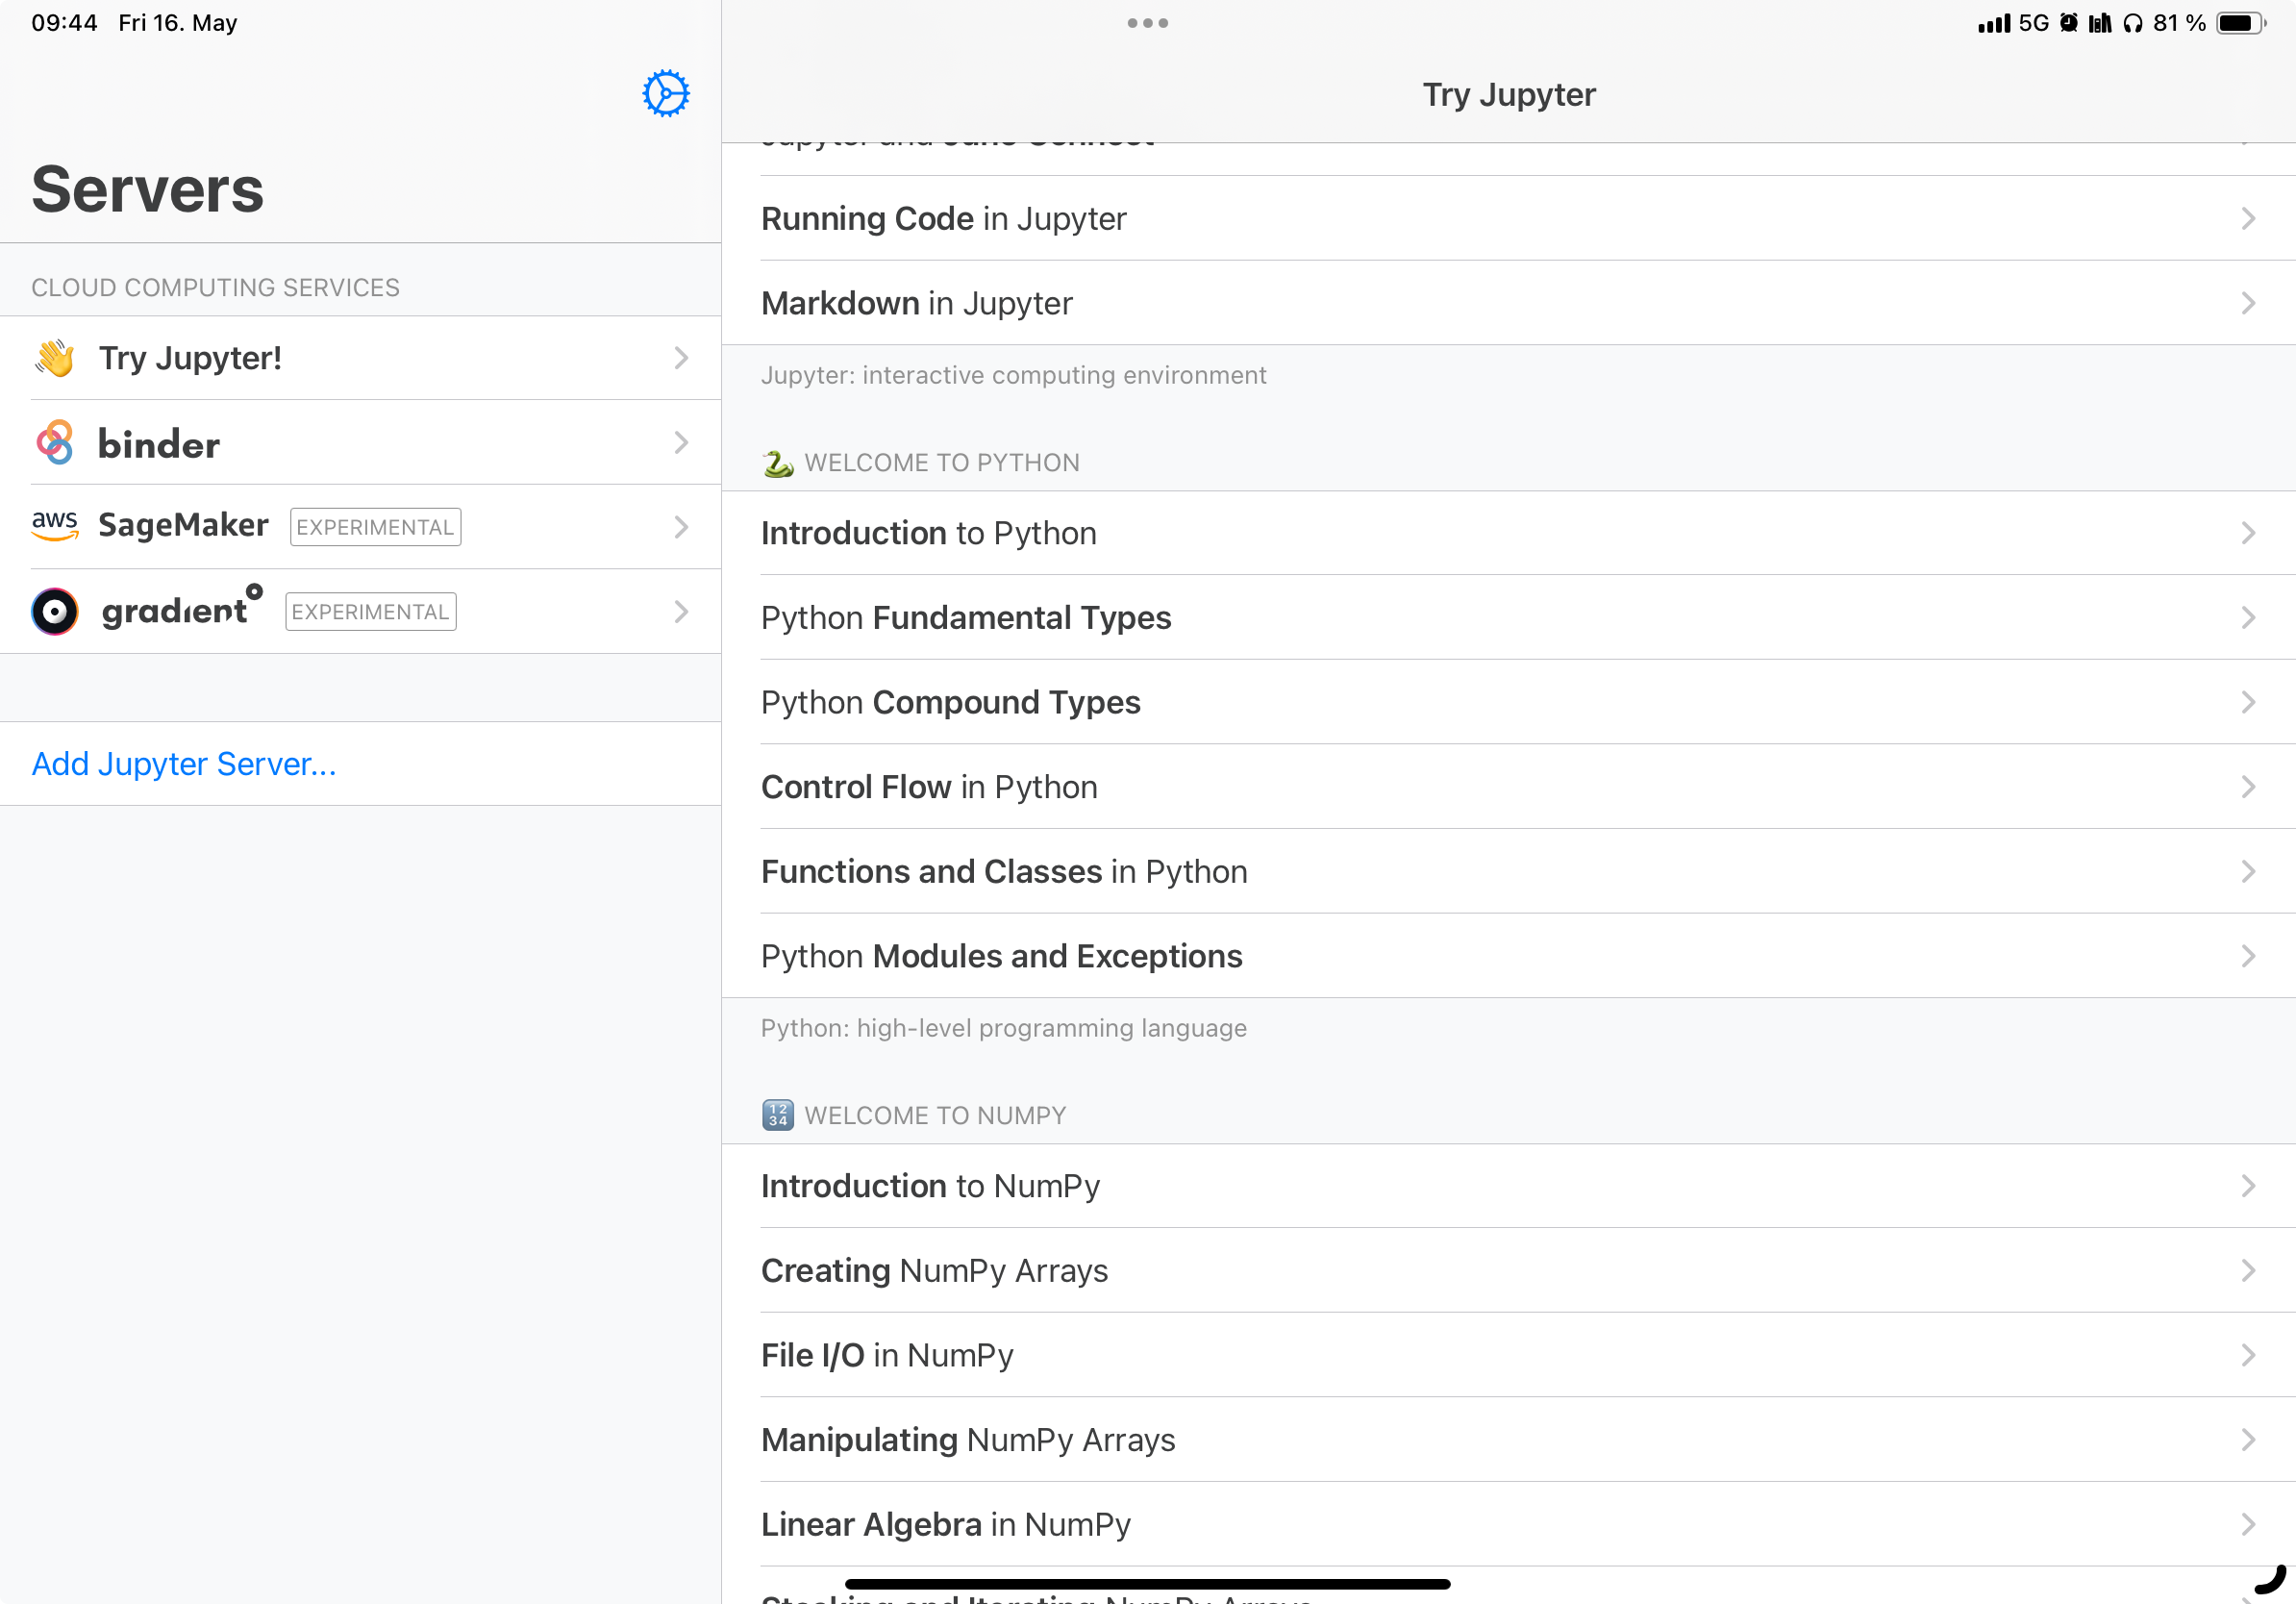
\includegraphics[scale = 0.1]{attachment/chapter_14/Scc001.png}
	\caption{Juno Conect}
\end{figure}

\paragraph{Allow Changes to the repo}
This will allow to execute and change in a cloud-based repo. The setting can be found in the personal settings (not repo settings)
\begin{figure}[H]
	\centering
	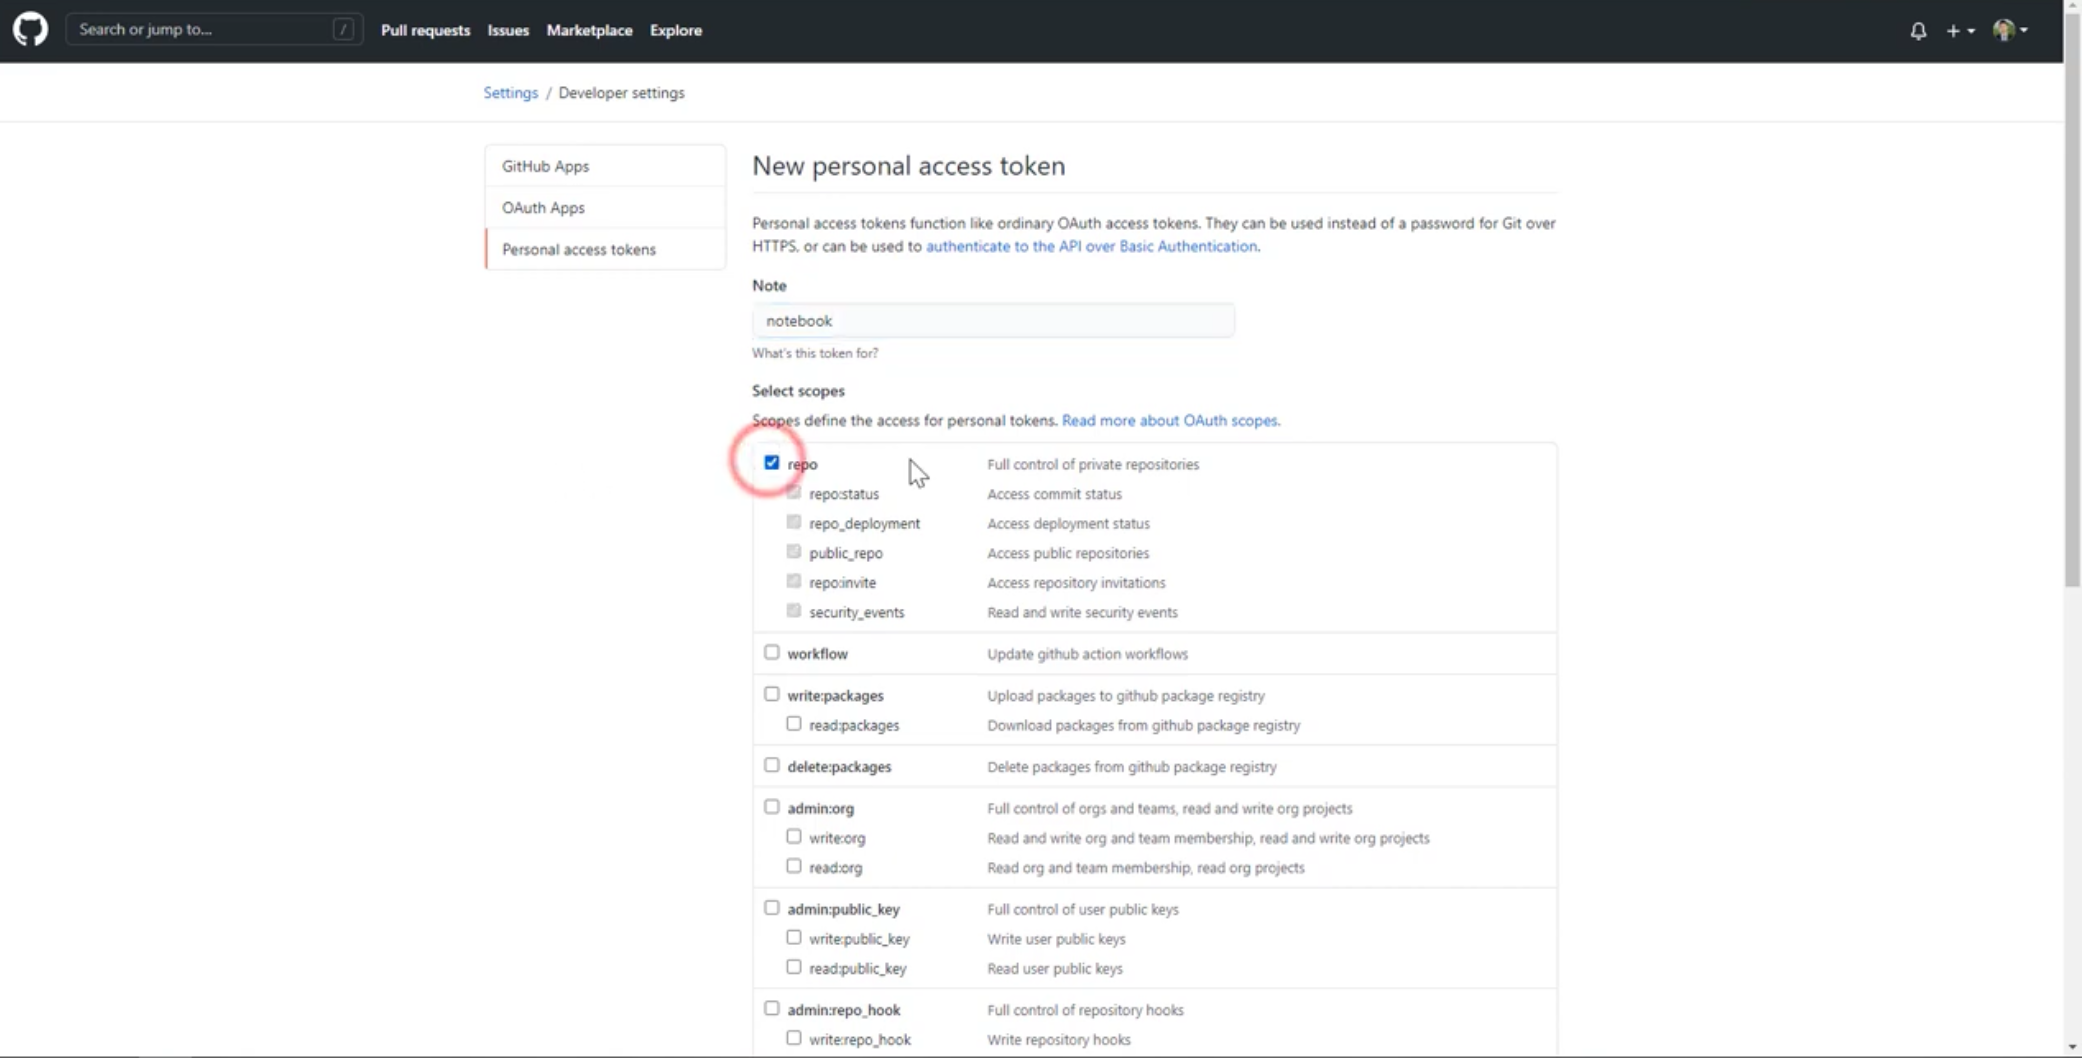
\includegraphics[scale = 0.1]{attachment/chapter_14/Scc002.png}
	\caption{Create Personal Token on GitHub}
\end{figure}

\paragraph{AWS: Create S3 Bucket} This creates a storage ressource.

\begin{figure}[H]
	\centering
	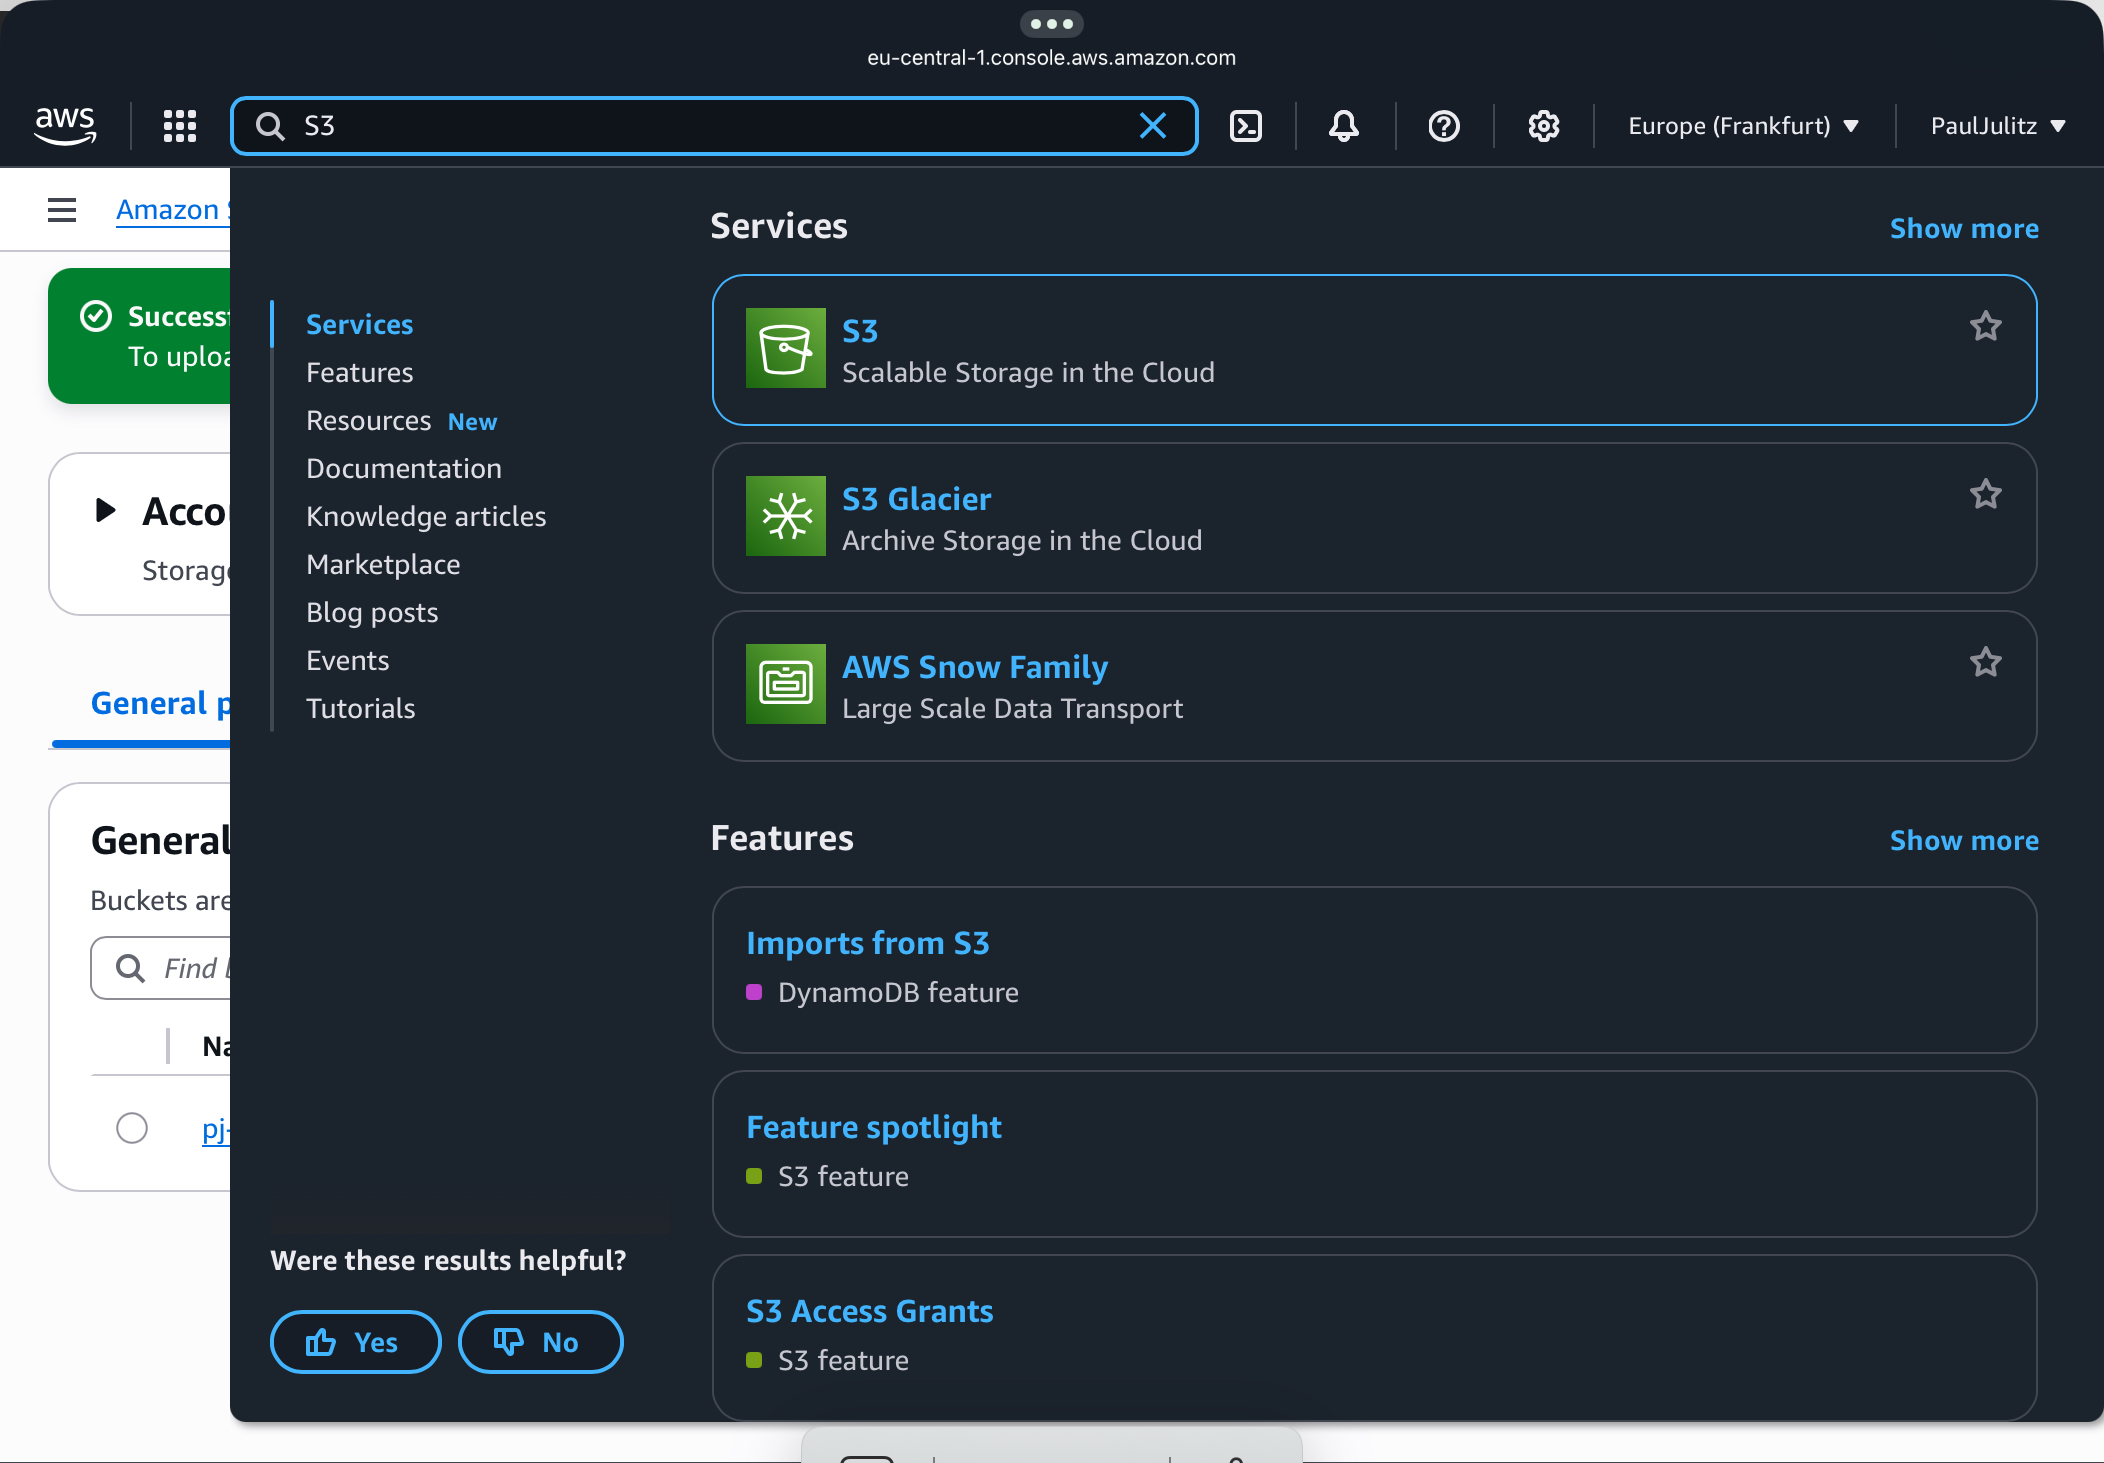
\includegraphics[scale = 0.1]{attachment/chapter_14/Scc003.png}
	\caption{Create a s3 data storage bucket}
\end{figure}

\paragraph{AWS: Create a role (IAM)}
This is a resource which identifiers and manages the access to the resources in AWS. We create a role with the name \textit{rl notebook}. For this we use \textbf{IAM}.

\begin{figure}[H]
	\centering
	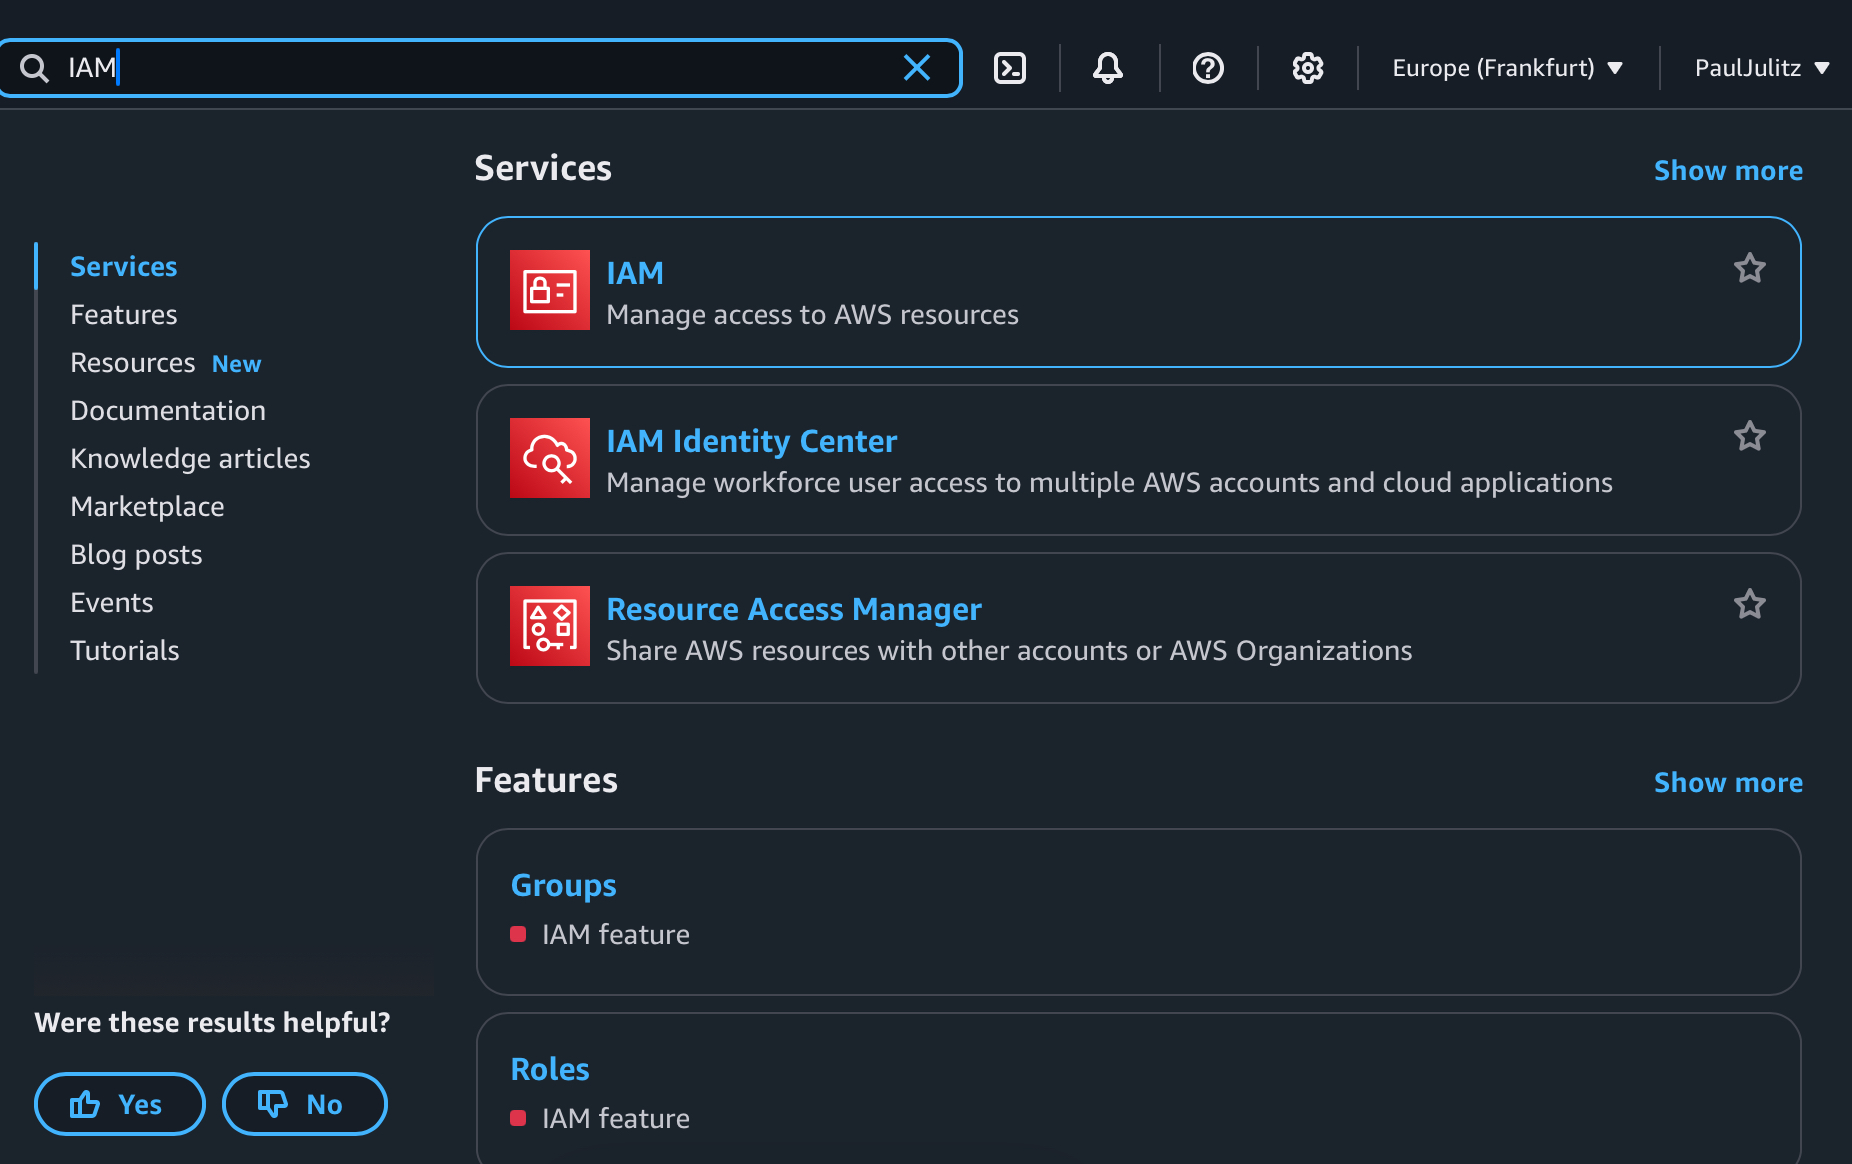
\includegraphics[scale = 0.1]{attachment/chapter_14/Scc004.png}
	\caption{Handeling the access to the ressources}
\end{figure}

We describe the use case for what we want to use the role.

\begin{figure}[H]
	\centering
	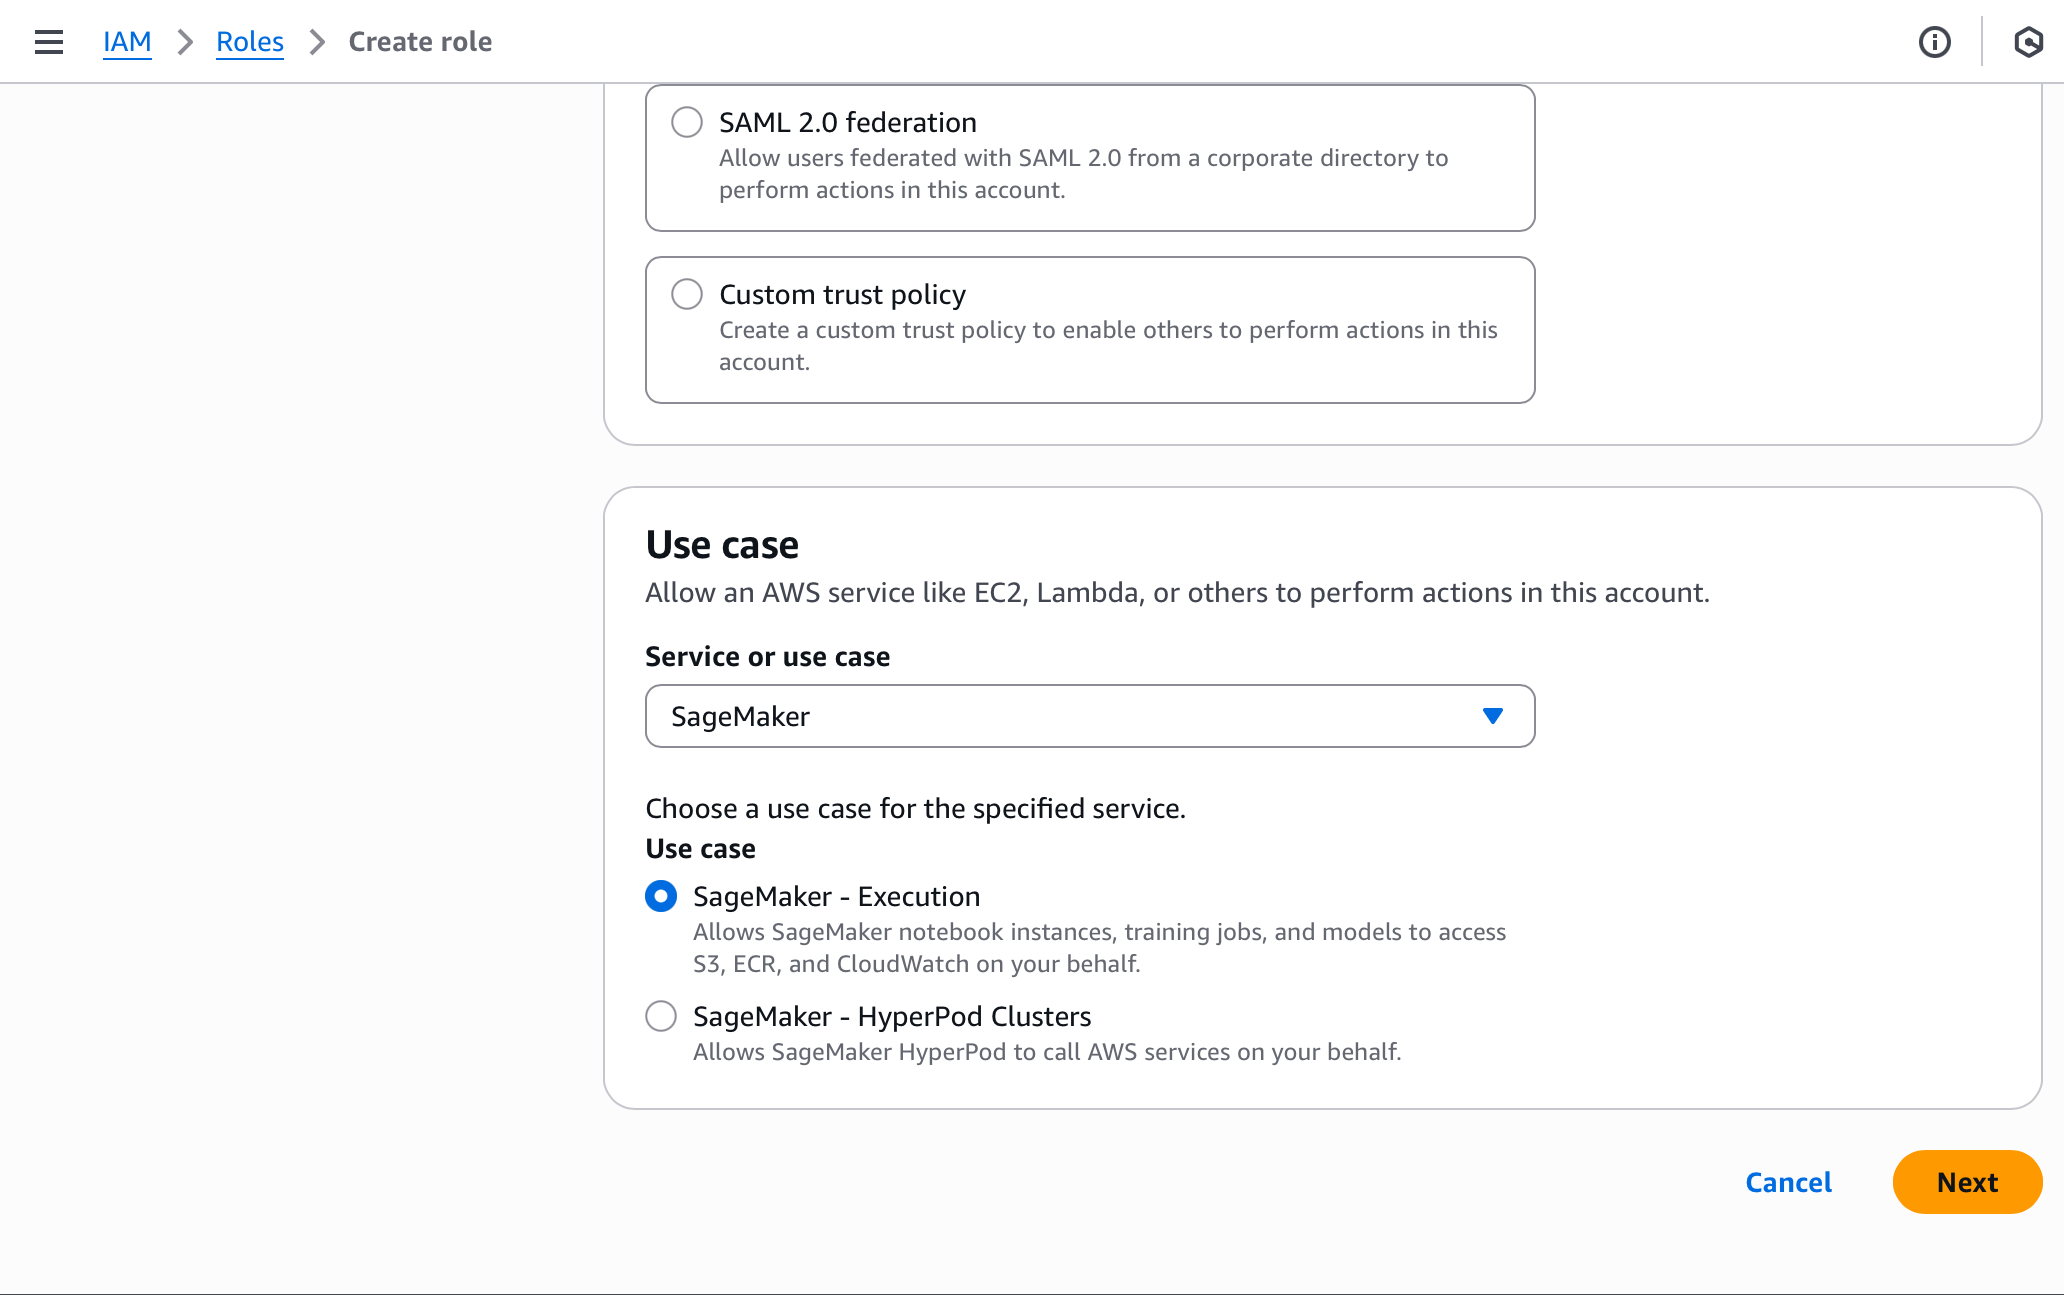
\includegraphics[scale = 0.1]{attachment/chapter_14/Scc005.png}
	\caption{Creating Role for SageMaker}
\end{figure}

Then we add more permission to the role.

\begin{figure}[H]
	\centering
	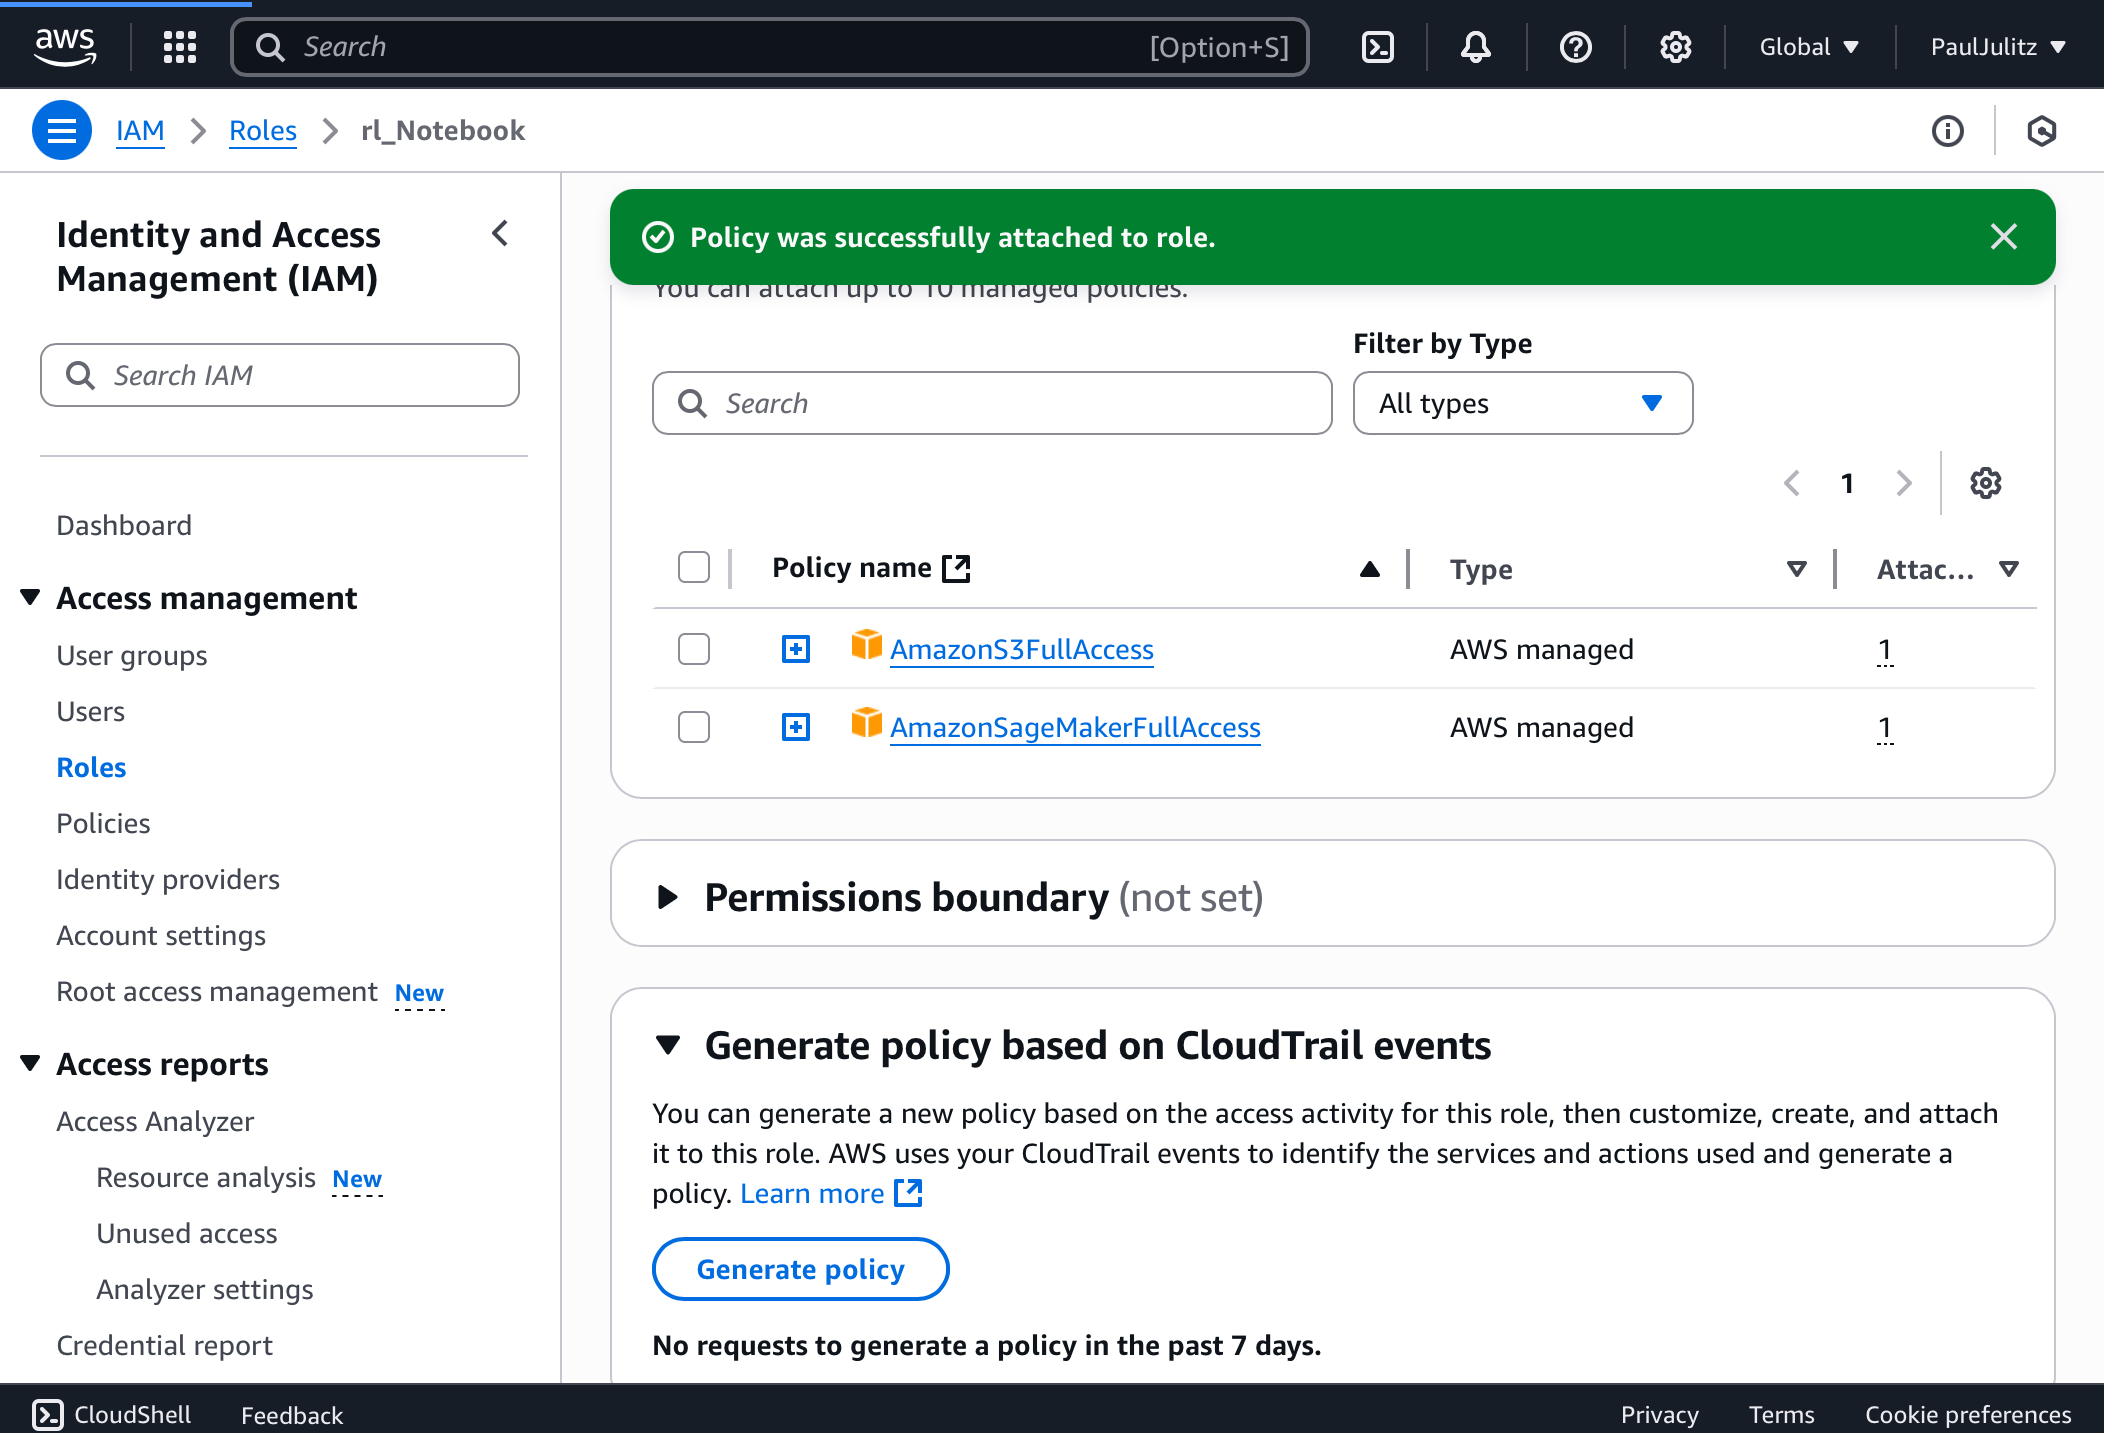
\includegraphics[scale = 0.1]{attachment/chapter_14/Scc006.png}
	\caption{Add S3 full access permission.}
\end{figure}


